\chapter{Literature Review}
 In this chapter, we review the foundations and advanced algorithms for shortest path calculations, including preprocessing techniques. The section spans classical algorithms, advanced algorithms and recent advances in graph-optimization.
\section{Classical shortest path algorithms}
	\subsection{Breadth-first Search}
		\subsubsection{Introduction}
		Breadth-first search is a graph traversal algorithms invented by Konrad Zuse in 1945, that can also be used to find the shortest path from a source vertex to a destination vertex in an unweighted graph.
		
		\subsubsection{Algorithm}
			\begin{enumerate}
				\item Mark all vertices as unvisited.
				\item Assign $distance[u] = \infty$ for all vertices except the source vertex $s$, where $distance[s] = 0$.
				\item Use a queue to track vertices to explore. Start with the source vertex $s$.
				\item Dequeue a vertex $u$.
				\item For each neighbour $v$ of $u$, If $v$ is unvisited (i.e., $distance[v]=\infty$):
					\begin{itemize}
						\item Set $distance[v] = distance[u] + 1$.
						\item Mark $v$ as visited.
						\item Enqueue $v$.
					\end{itemize}
				\item The algorithm ends when the queue is empty. Unreachable vertices retain $distance = \infty$.
			\end{enumerate}
			This algorithm is mathematically predisposed to find the shortest path from a source vertex $s$ to every other vertex in the graph (see\textbf{ Appendix \ref{appendix:bfs:correctness}} for a formal proof).
		
		\subsubsection{Complexity}
			When finding the shortest path between a pair of vertices in a graph, the worst-case time complexity for the BFS algorithm is $O(V)$ for queue operations + $O(E)$ for edge processing, netting a worst-case time complexity of $O(V + E)$ (see \textbf{Appendix \ref{appendix:bfs:complexity}} for a formal proof). \\ \\
			The space complexity for BFS is $O(V)$ since we use a queue to store the vertices yet to be explored.
		
		\subsubsection{Pros and Cons}
			\begin{itemize}
				\item The algorithm is simple and efficient for unweighted graphs.
				\item BFS works well for large, sparse graphs.
				\item BFS fails for shortest-path problems in weighted graphs, which are more useful when modelling real world scenarios.
			\end{itemize}
	\subsection{Bellman-ford Algorithm}
		\subsubsection{Introduction}
			The Bellman–Ford algorithm is a shortest-path algorithm that utilizes dynamic programming to compute shortest paths from a single source vertex to all of the other vertices in a weighted, directed graph. It was first published by Richard Bellman (1958) and Lester Ford Jr. (1956), hence its name.
		\subsubsection{Algorithm}
			\begin{enumerate}
				\item Create an array $distance$ of size $V$ to store the shortest path distances.
				\item Assign $distance[u] = \infty$ for all vertices except the source vertex $s$, where $distance[s] = 0$.
				\item Repeat $V - 1$ times:
					\begin{itemize}
						\item For each edge $(u,v) \in E$, if $distance[u] + w(u,v) < distance[v]$ update $distance[v]=distance[u]+w(u,v)$.
					\end{itemize}
				\item Now to detect a negative cycle, for each edge $(u,v) \in E$, if $distance[u] + w(u,v) < distance[v]$, report that a negative-weight cycle exists.
				\item If no negative-weight cycle is detected, Return the $distance$ array as the shortest path distances.
			\end{enumerate}
			Refer to \textbf{Appendix \ref{appendix:bellford:correctness}} for a formal proof of correctness of this algorithm.
		\subsubsection{Complexity}
			When finding the shortest path between a pair of vertices in a graph, the worst-case time complexity for the Bellman-Ford algorithm is $O(V \cdot E)$ (see \textbf{Appendix \ref{appendix:bellford:complexity}} for a formal proof). \\ \\
			The space complexity for Bellman-Ford is $O(V)$ since we use an array of size $V$ to store all the shortest-path distances.
		\subsubsection{Pros and Cons}
			\begin{itemize}
				\item Suitable for applications requiring negative weight handling, in which case it can detect the existence of a negative cycle.
				\item The Bellman-Ford algorithm is more complex than Dijkstra's algorithm.
				\item Much slower compared to Dijkstra's algorithm.
			\end{itemize}
	\subsection{Dijkstra's Algorithm}
		\subsubsection{Introduction}
		
		\subsubsection{Algorithm}
		\begin{enumerate}
			\item 
			\item 
			\item 
			\item 
			\item 
		\end{enumerate}
		
		\subsubsection{Complexity}
		
		\subsubsection{Pros and Cons}
		\begin{itemize}
			\item 
			\item 
			\item
		\end{itemize}
		

\section{Advanced shortest path algorithms}
\subsection{A* Search Algorithm}
\subsection{Bidirectional Search}

\section{Preprocessing techniques}
\subsection{Contraction Hierarchies}
\subsection{ALT Algorithm}
\subsection{Hub Labeling}

Refer figure \ref{fig:label}.

\section{Summary of Findings}
%\begin{figure}[htb]
%\centering
%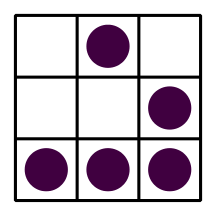
\includegraphics[scale=0.3]{./glider} % e.g. insert ./image for image.png in the working directory, adjust scale as necessary
%\caption{Caption here}
%\label{fig:label} % insert suitable label, this is used to refer to a fig from within the text as shown above
%\end{figure}

\section{Gaps in current approaches}
	\begin{itemize}
		\item Limited scalability in dynamic graphs.
		\item Lack of flexibility for user preferences.
		\item High preprocessing overhead in large graphs.
	\end{itemize}

